% no answer key
% \documentclass[letterpaper]{exam}

% answer key
\documentclass[letterpaper, landscape]{exam}
\usepackage{2in1, lscape} 
\printanswers


\usepackage{units} 
\usepackage{xfrac} 
\usepackage[fleqn]{amsmath}
\usepackage{cancel}
\usepackage{float}
\usepackage{mdwlist}
\usepackage{booktabs}
\usepackage{cancel}
\usepackage{polynom}
\usepackage{caption}
\usepackage{fullpage}
\usepackage{comment}
\usepackage{enumerate}
\usepackage{graphicx}
\usepackage{parskip}

\everymath{\displaystyle}


\title{Statistics \\ Homework Five}
\date{\today}
\author{}

\begin{document}

  \maketitle

  \section{Homework}
    \begin{itemize*}
      \item read Chapter 5 
      \item take a look at the ``Check Your Skills'' exercises
      \item exercises: 
    \end{itemize*}

  \ifprintanswers
  \else
    Here are the calculations for problems which require an expensive
    calculator.

    \begin{description}
      \item[34] .

        \begin{tabular}[H]{lr}
          \toprule
          slope     & 0.527 \\
          intercept & 27.635 \\
          $r^2$     & 0.3114 \\
          \bottomrule
        \end{tabular}

      \item[37] .

        \begin{tabular}[H]{lrr}
          \toprule
                    & With Outlier & Without Outlier \\
          \midrule
          slope     & 0.0088       & 0.0089 \\
          intercept & 0.5850       & 0.5858 \\
          $r^2$     & 0.7201       & 0.4920 \\
          \bottomrule
        \end{tabular}

      \item[38]
        All the data sets have about the same numbers:

        \begin{tabular}[H]{lr}
          \toprule
          slope     & 0.5   \\
          intercept & 3.0   \\
          $r^2$     & 0.666 \\
          \bottomrule
        \end{tabular}
    \end{description}
  \fi

  \ifprintanswers
    \begin{description}

      \item[27]     
        \begin{figure}[H]
          \centering
          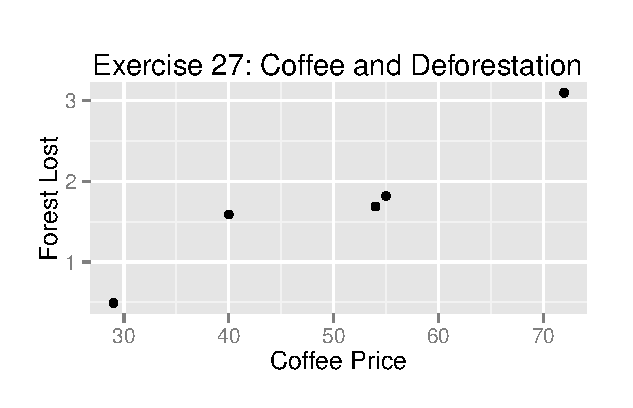
\includegraphics{figures/ex27.eps}
          \caption{Exercise 27}
        \end{figure}

        \begin{parts}
          \part $m = \unit[0.0138]{m/s}$  Every 0.0138 meters of dive depth takes the
          penguin another second of dive time.

        \part 
          \[
            DD(200) = 2.69 + 0.0138 \cdot 200 \approx \unit[5.45]{s}
          \]
        \end{parts}
    
      \item[28]
        \begin{parts}
          \part for every $\unit[1.507]{mg/l}$ increase in the concentration of TOC,
            there is a $\unit[1]{mg/l}$ increase in the concentration of BOD.

          \part The predicted value is $\unit[-55.43]{mg/l}$.  Perhaps nothing can
            live when the total organic carbon is close to zero, so the BOD value
            doesn't make sense.
        \end{parts}

      \item[30]
        \begin{parts}
          \part 
            \begin{align*}
              y &= 157.68 - 2.993 x \\
              y(30) &= 67.88 \% \\
            \end{align*}

          \part From Figure 5.11, $r^2 = 63.1 \%$
            
          \part Since the correlation coefficient doesn't depend on the order,
          it would be the same magnitude and sign.  The line slopes down, so the
          correlation coefficient is negative:
          \[
            r = - \sqrt{67.88} = -8.24
          \]

        \end{parts}

      \item[31]
        \begin{parts}
          \begin{align*}
            b  & = 0.5 \cdot \frac{2.8}{2.7} \\
               & = 0.5185
            \\
            a  & = 69 - 0.5185 \cdot 64 \\
               & = 35.82 \\
          \end{align*}

          The equation is:
          \[
            \hat{y} = 35.82 + 0.5185 \hat{x}
          \]

          \part
            \begin{figure}[H]
              \centering
              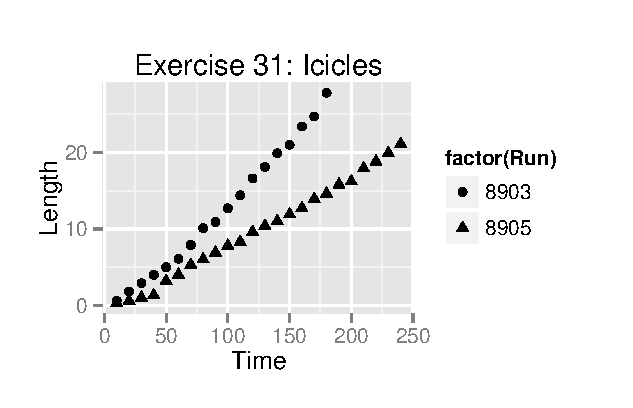
\includegraphics{figures/ex31.eps}
              \caption{Exercise 31}
            \end{figure}

          \part The estimate isn't very accurate:
            \[
              r^2 = 0.5^2 = 0.25
            \]

            The height relationship only accounts for about 25\% of the variation
            in the heights.
            
        \end{parts}

      \item[32]
        \begin{parts}
          \part
            \begin{align*}
              a & = 0.6 \cdot \frac{75}{280} \\
                & = 0.1607 \\
            \end{align*}

            \begin{align*}
              75 & = 0.1607 \cdot 280 + b \\
              b  & = 30.04 \\
            \end{align*} 

            The equation is:
            \[
              \hat{y} = 30.04 + 0.1607 x
            \]

          \part 
            \[
              y(300) = 78.25
            \]

          \part
            $r^2 = 0.36$.  The earlier scores only account for 36\% of the
            variation in the final score. 
        \end{parts}

      \item[33]
        \begin{align*}
          r^2 & = 0.16 \\
          r   & = 0.4 \\
        \end{align*}

        $r$ is positive because the more classes you attend, the better your
        grade.

      \item[34]
        \begin{parts}
          \part 
            $y = 0.527x + 27.635$
            \begin{figure}[H]
              \centering
              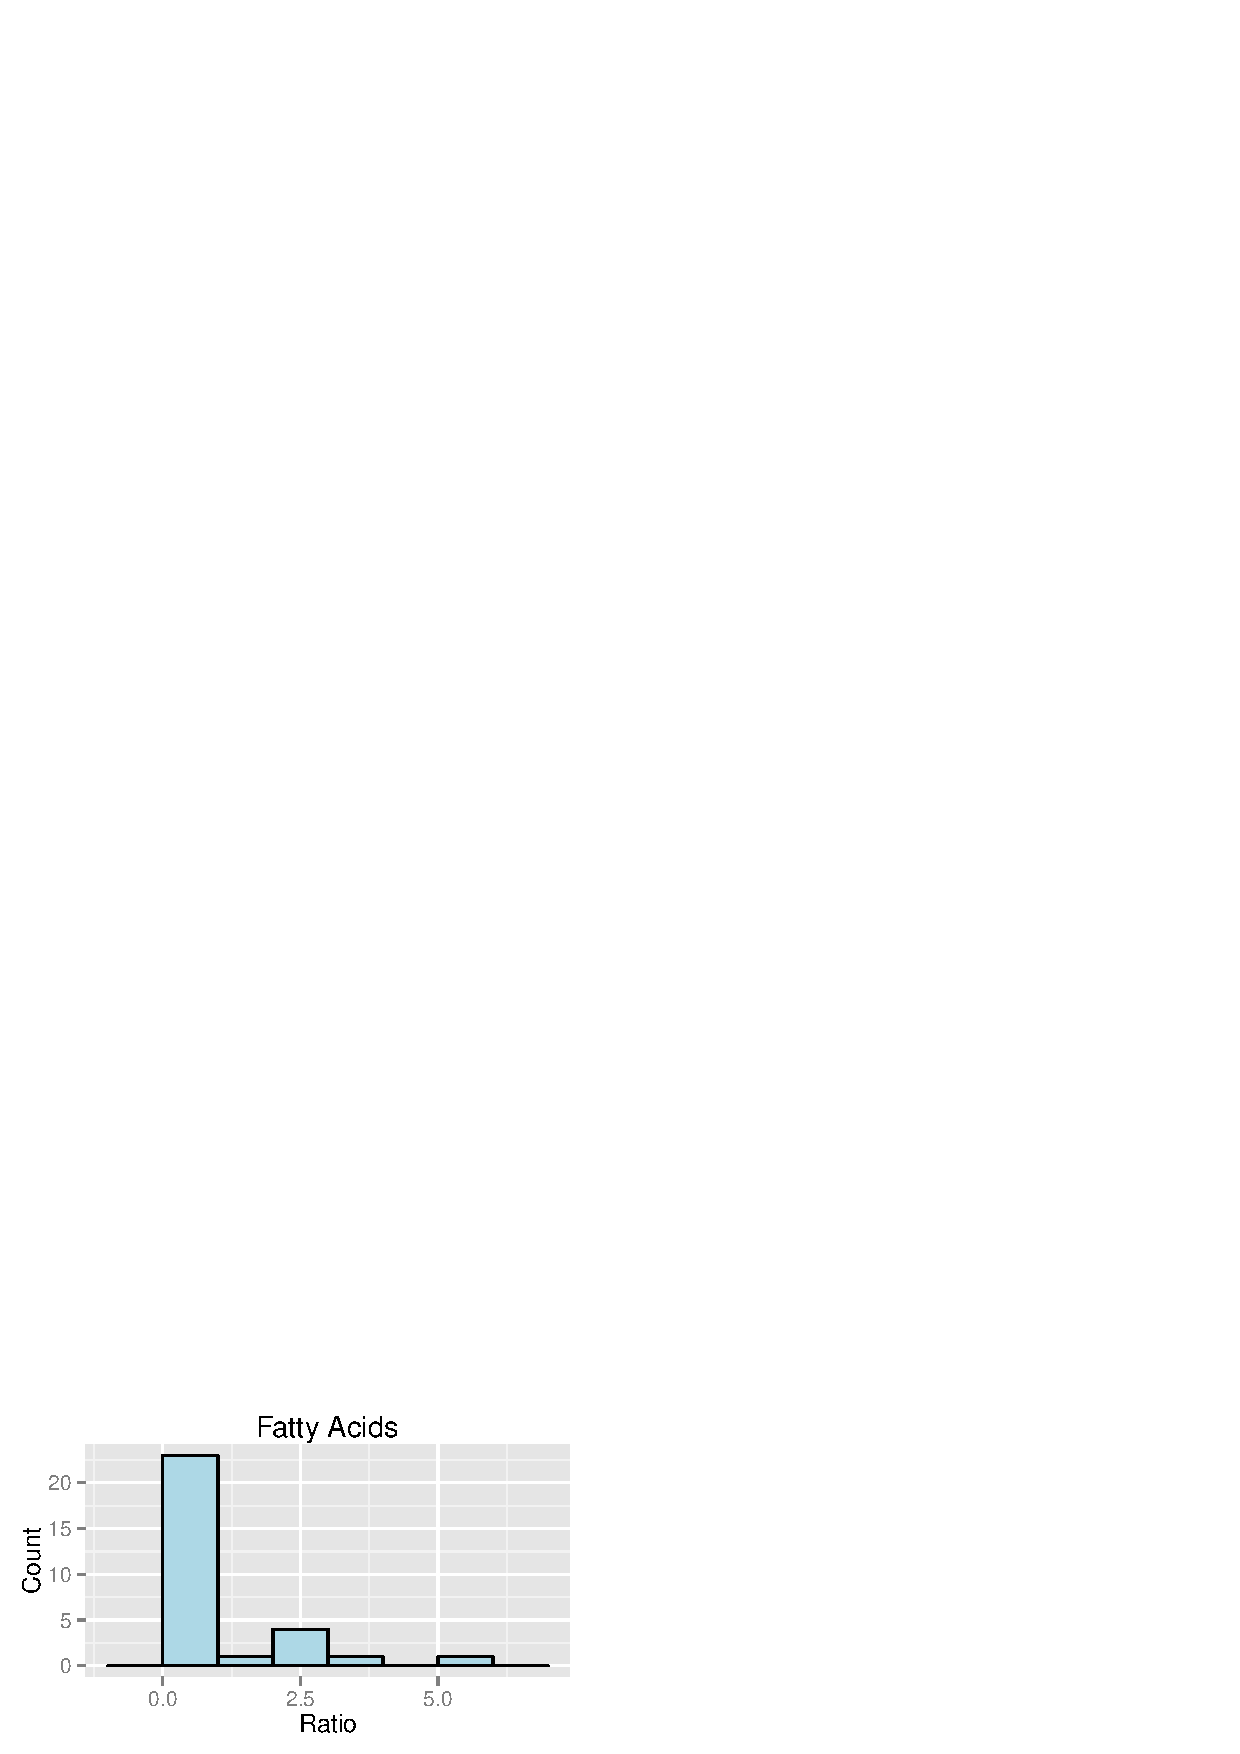
\includegraphics{figures/ex34.pdf}
              \caption{Exercise 34}
            \end{figure}

          \part
            According to the model, Tonya will be about 65 inches tall.  Since
            $r^2$ is only 0.3114, the model only explains 31\% of the variation
            so the prediction probably won't be very accurate.
        \end{parts}

      \item[37]
        \begin{description}
          \item[a-b]
            \begin{figure}[H]
              \centering
              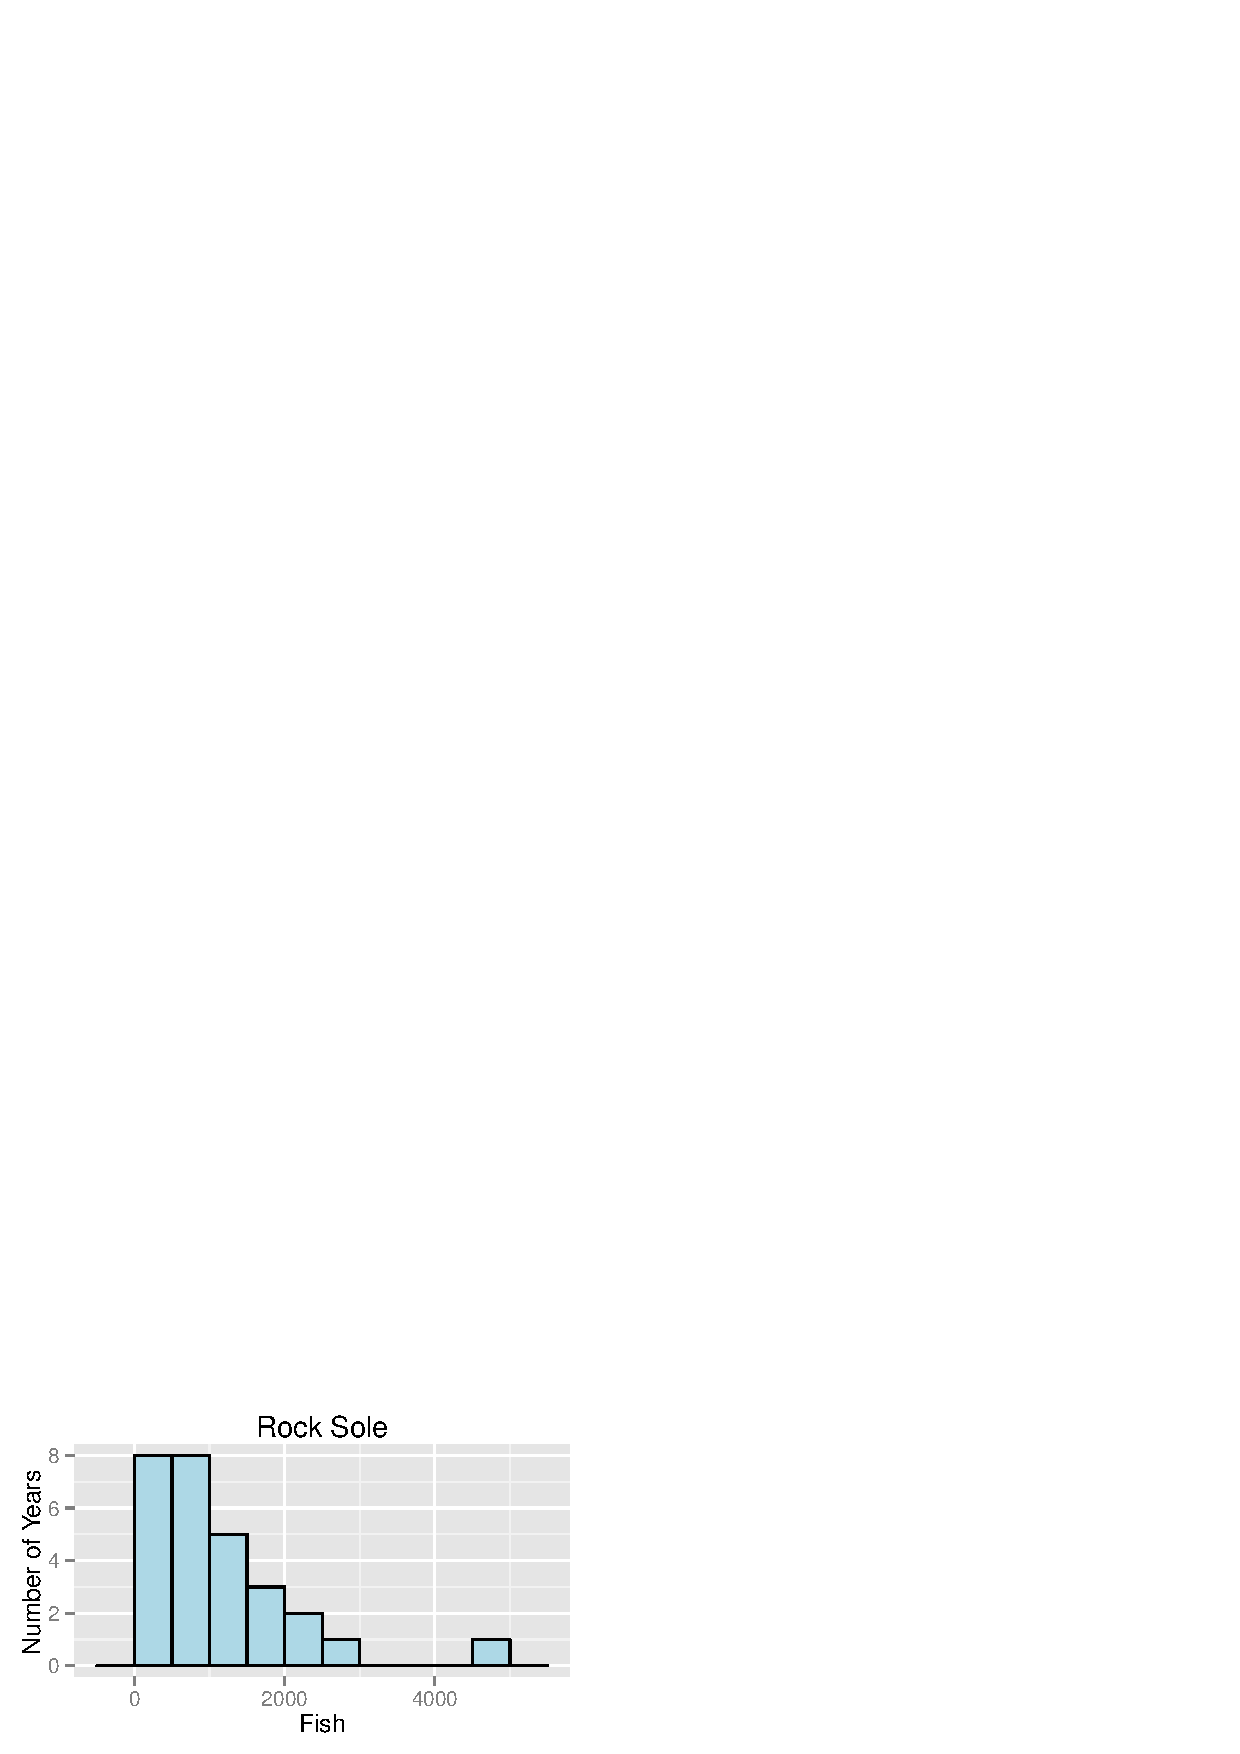
\includegraphics{figures/ex37.pdf}
              \caption{Exercise 37}
            \end{figure}

          \item[c]
            The outlier increases the correlation because it adds a term
            with a high value in both the x and y dimensions.  The outlier
            doesn't affect the regression line much because it is exactly on the
            regression line.

          \item[d]
            \begin{tabular}[H]{lrr}
              \toprule
                        & With Outlier & Without Outlier \\
              \midrule
              slope     & 0.0088       & 0.0089 \\
              intercept & 0.5850       & 0.5858 \\
              $r$       & 0.8486       & 0.7015 \\
              \bottomrule
            \end{tabular}
        \end{description}

      \item[38]
        \begin{figure}[H]
          \centering
          \includegraphics{figures/ex38a.pdf}
          \caption{Exercise 38 (a)}
        \end{figure}

        \begin{figure}[H]
          \centering
          \includegraphics{figures/ex38b.pdf}
          \caption{Exercise 38 (b)}
        \end{figure}

        \begin{figure}[H]
          \centering
          \includegraphics{figures/ex38c.pdf}
          \caption{Exercise 38 (c)}
        \end{figure}

        \begin{figure}[H]
          \centering
          \includegraphics{figures/ex38d.pdf}
          \caption{Exercise 38 (d)}
        \end{figure}

        \begin{description}
          \item[a]
            All of the data sets are about the same.
            \begin{align*}
              y & = 0.5 x + 3 \\
              r & \approx 0.816 \\
            \end{align*}

          \item[c]
            \begin{itemize*}
              \item Graph a looks like a linear relationship, with some minor
                variations.

              \item Graphs b and d don't look like linear relationships.

              \item Graph c looks like a linear relationship with one outlier.
                I would discard the outlier and compute a new regression line.
                It looks like the outlier is drawing the line away from
                where it should be.
            \end{itemize*}
      \end{description}

      \item[42]
        People use artificial sweeteners because they are already overweight, so
        weight is causing the sweetener use rather than the other way around.

    \end{description}

  \else
    \vspace{10 cm}
    \begin{quote}
      \begin{em}
        The more corrupt a society, the more numerous its laws.
      \end{em}
    \end{quote}
    \hspace{1 cm} --Edward Abbey
  \fi

\end{document}

